\subsection{Laurent展開}
	
	いま$R$を正の実数とし,$f$を
	\begin{align}
		\Omega \defeq \disc{0}{R} \backslash \{0\}
	\end{align}
	上の正則関数とする.また$z$を$\Omega$の要素とし,$r$と$\rho$を
	\begin{align}
		r < |z| < \rho < R
	\end{align}
	を満たす正の実数とする.このとき
	\begin{align}
		[0,1] \ni t \longmapsto \rho \cdot e^{2 \cdot \pi \cdot \isym \cdot t}
	\end{align}
	なる路を$\gamma$とし,
	\begin{align}
		[0,1] \ni t \longmapsto r \cdot e^{2 \cdot \pi \cdot \isym \cdot t}
	\end{align}
	なる路を$\eta$とすれば,
	\begin{align}
		f(z) = \frac{1}{2 \cdot \pi \cdot \isym} \cdot 
		\left[-\int_{\eta} \frac{f(\zeta)}{\zeta}\ d\zeta + \int_{\gamma} \frac{f(\zeta)}{\zeta}\ d\zeta\right]
		\label{fom:Laurent_series_1}
	\end{align}
	が成立する.
	
	細かいところは後に回して概略を説明する.いま
	\begin{align}
		\alpha \defeq \pvarg{z} + \pi
	\end{align}
	及び
	\begin{align}
		\beta \defeq \frac{\alpha}{2 \cdot \pi}
	\end{align}
	とおき,$\theta$を$\eta$の逆路とし,$[0,4]$上の路$\xi$を
	\begin{align}
		t \longmapsto
		\begin{cases}
			\gamma(t) & \mbox{if } 0 \leq t \leq \beta \\
			\seg{\rho \cdot e^{\isym \cdot \alpha}}{r \cdot e^{\isym \cdot \alpha}}(t-\beta) & \mbox{if } \beta \leq t \leq \beta + 1 \\
			\theta(t - \beta - 1) & \mbox{if } \beta + 1 \leq t \leq \beta + 2 \\
			 \seg{r \cdot e^{\isym \cdot \alpha}}{\rho \cdot e^{\isym \cdot \alpha}}(t-\beta) & \mbox{if } \beta + 2 \leq t \leq \beta + 3 \\
			\gamma(t - \beta - 3) & \mbox{if } \beta + 3 \leq t \leq 4
		\end{cases}
	\end{align}
	なる関係により定める.イメージとしては,$\xi$は始め
	
	\begin{center}
		\begin{tikzpicture}
			\node [anchor=north] at (0,0) {$0$};
			\node [anchor=west] at ({sqrt(2)},{sqrt(2)}) {$z$};
			\draw [domain=0:2*pi, samples=200, dotted] plot({3*cos(\x r)},{3*sin(\x r)});
			\foreach \Point in {({sqrt(2)},{sqrt(2)})}{
				\node at \Point {\textbullet};
			}
			\draw [domain=0:(5*pi/4), thick, samples=200, color=red] plot({2.5*cos(\x r)},{2.5*sin(\x r)});
			\draw [thick, color=red, ->] ({-2.5/sqrt(2)},{-2.5/sqrt(2)}) -- ({-1/sqrt(2)},{-1/sqrt(2)});
			
			\draw [domain=0:(5*pi/4), samples=200, ->] plot({0.5*cos(\x r)},{0.5*sin(\x r)});
			\draw [dotted] (0,0) -- (2.5,0);
			\draw [dotted] ({sqrt(2)},{sqrt(2)}) -- ({-2.5/sqrt(2)},{-2.5/sqrt(2)});
			\node [anchor=north west] at ({cos(3*pi/4 r)},{sin(3*pi/4 r)}) {$\alpha$};
		\end{tikzpicture}
	\end{center}
	
	を描き,次は
	
	\begin{center}
		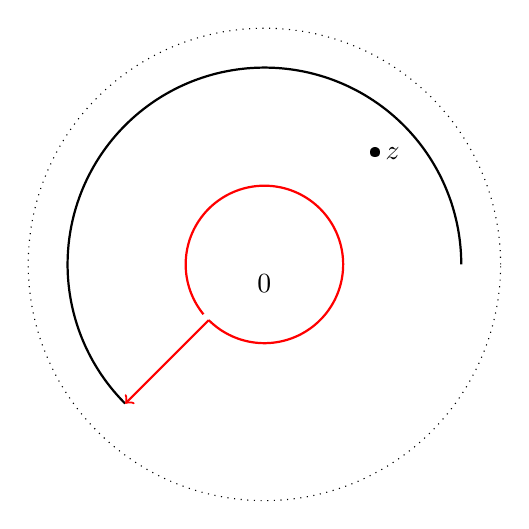
\begin{tikzpicture}
			\node [anchor=north] at (0,0) {$0$};
			\node [anchor=west] at ({sqrt(2)},{sqrt(2)}) {$z$};
			\draw [domain=0:2*pi, samples=200, dotted] plot({3*cos(\x r)},{3*sin(\x r)});
			\foreach \Point in {({sqrt(2)},{sqrt(2)})}{
				\node at \Point {\textbullet};
			}
			\draw [domain=0:(5*pi/4), thick, samples=200] plot({2.5*cos(\x r)},{2.5*sin(\x r)});
			\draw [domain=5*pi/4 - 0.1:-3*pi/4, thick, color=red, samples=200] plot({cos(\x r)},{sin(\x r)});
			\draw [thick, color=red, ->] ({-1/sqrt(2)},{-1/sqrt(2)}) -- ({-2.5/sqrt(2)},{-2.5/sqrt(2)});
		\end{tikzpicture}
	\end{center}
	
	を描き,最後に
	
	\begin{center}
		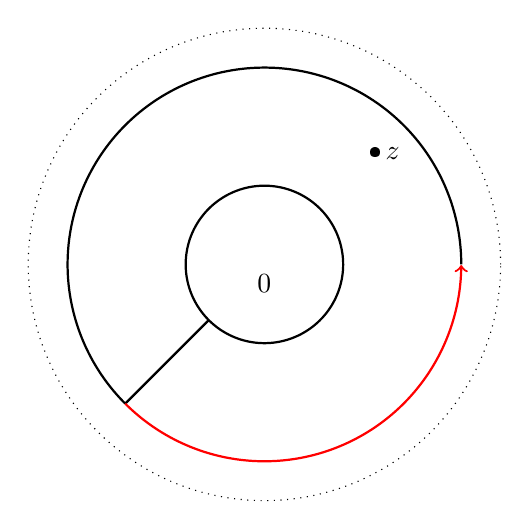
\begin{tikzpicture}
			\node [anchor=north] at (0,0) {$0$};
			\node [anchor=west] at ({sqrt(2)},{sqrt(2)}) {$z$};
			\draw [domain=0:2*pi, samples=200, dotted] plot({3*cos(\x r)},{3*sin(\x r)});
			\foreach \Point in {({sqrt(2)},{sqrt(2)})}{
				\node at \Point {\textbullet};
			}
			\draw [domain=0:(5*pi/4), thick, samples=200] plot({2.5*cos(\x r)},{2.5*sin(\x r)});
			\draw [thick] ({-2.5/sqrt(2)},{-2.5/sqrt(2)}) -- ({-1/sqrt(2)},{-1/sqrt(2)});
			\draw [domain=(-3*pi/4):(5*pi/4), thick, samples=200] plot({cos(5*pi/4-\x r)},{sin(5*pi/4-\x r)});
			\draw [thick] ({-1/sqrt(2)},{-1/sqrt(2)}) -- ({-2.5/sqrt(2)},{-2.5/sqrt(2)});
			\draw [domain=(5*pi/4):2*pi, thick, color=red, samples=200, ->] plot({2.5*cos(\x r)},{2.5*sin(\x r)});
		\end{tikzpicture}
	\end{center}
	
	を描く.
	
	\begin{screen}
		\begin{thm}[線積分の微分積分学の基本定理]
			$\Omega$を$\C$の開集合とし,$f$を$\Omega$上の正則関数とし,
			$\gamma$を$[0,1]$から$\Omega$への路とする.このとき
			\begin{align}
				\int_{\gamma} f' = f(\gamma(1)) - f(\gamma(0)).
			\end{align}
		\end{thm}
	\end{screen}
	
	\begin{sketch}
		$\epsilon$を任意に与えられた正の実数とし,
		\begin{align}
			L \defeq |\mu_{\gamma}|([0,1])
		\end{align}
		とおき,
		\begin{align}
			r \defeq \inf{}{\Set{|\gamma(t) - z|}{t \in [0,1] \wedge z \in \C \backslash \Omega}}
		\end{align}
		とおく.このとき
		\begin{align}
			N \defeq \bigcup_{t \in [0,1]} \disc{\gamma(t)}{r/2}
		\end{align}
		とおけば,$\overline{N}$はコンパクトであって
		\begin{align}
			\overline{N} \subset \Omega
		\end{align}
		を満たし,$f'$は$\overline{N}$の上で連続であるから,
		\begin{align}
			\delta < \frac{r}{2}
		\end{align}
		なる正の実数$\delta$で
		\begin{align}
			\forall z,w \in \overline{N}\,
			\left[\, |z-w| < \delta \Longrightarrow |f'(z) - f'(w)| < \frac{\epsilon}{L}\, \right]
		\end{align}
		を満たすもの取れる.一方で,自然数$n$で
		\begin{align}
			\left|\int_{[0,1]} f' \circ \gamma\ d\mu_{\gamma}
			- \sum_{k=0}^{n-1} f'(\gamma(k/n)) \cdot \left(\gamma((k+1)/n) - \gamma(k/n)\right)\right|
			< \epsilon
		\end{align}
		及び,$n$より小さい任意の自然数$k$に対して
		\begin{align}
			|\gamma((k+1)/n) - \gamma(k/n)| < \delta
		\end{align}
		を満たすものが取れる.ここで
		\begin{align}
			[0,1] \ni t \longmapsto \sum_{k=0}^{n-1} \gamma(k/n) + \frac{t - k/n}{1/n} \cdot \left(\gamma((k+1)/n) - \gamma(k/n)\right)
		\end{align}
		なる路を$\eta$とおけば,微分積分学の基本定理より
		\begin{align}
			\int_{[0,1]} f' \circ \eta\ d\mu_{\eta} = f(\eta(1)) - f(\eta(0))
			= f(\gamma(1)) - f(\gamma(0))
		\end{align}
		が成り立ち,他方で
		\begin{align}
			&\left|\int_{[0,1]} f' \circ \eta\ d\mu_{\eta}
			- \sum_{k=0}^{n-1} f'(\gamma(k/n)) \cdot \left(\gamma((k+1)/n) - \gamma(k/n)\right)\right| \\
			&= \left|\sum_{k=0}^{n-1} \int_{\left(\frac{k}{n},\frac{k+1}{n}\right]} f' \circ \eta\ d\mu_{\eta}
			- \sum_{k=0}^{n-1} \int_{\left(\frac{k}{n},\frac{k+1}{n}\right]} f'(\eta(k/n))\ d\mu_{\eta}\right| \\
			&\leq \sum_{k=0}^{n-1} \int_{\left(\frac{k}{n},\frac{k+1}{n}\right]}
			\left|f' \circ \eta - f'(\eta(k/n))\right|\ d|\mu_{\eta}| \\
			&\leq \frac{\epsilon}{L} \cdot \sum_{k=0}^{n-1} |\mu_{\eta}|\left(\left(k/n,(k+1)/n\right]\right) \\
			&= \frac{\epsilon}{L} \cdot \sum_{k=0}^{n-1} \left|\gamma((k+1)/n) - \gamma(k/n)\right| \\
			&\leq \epsilon
		\end{align}
		が成立する.以上から
		\begin{align}
			\left|\int_{[0,1]} f'\circ\gamma\ d\mu_{\gamma}
			- \left[f(\gamma(1)) - f(\gamma(0))\right]\right|
			\leq 2 \cdot \epsilon
		\end{align}
		が従い,$\epsilon$の任意性から
		\begin{align}
			\int_{[0,1]} f'\circ\gamma\ d\mu_{\gamma} = f(\gamma(1)) - f(\gamma(0))
		\end{align}
		が得られる.
		\QED
	\end{sketch}